\subsection{Реализация алгоритма трилатерации, основанном на пересечении сфер}

В геометрии трёхмерная проблема трилатерации представляет собой нахождение координат точки пересечения трёх сфер, которые определяются путём решения системы уравнений. Чтобы упростить вычисления, полагаем, что центры всех трех сфер лежат в плоскости $z=0$, один из них совпадает с началом координат, второй — лежит на оси $x$. Наложенные ограничения не уменьшают общности: к такому виду может быть приведена любая система соответствующих уравнений путем перехода к другой системе координат. Чтобы найти решение в исходной системе координат, к решению, найденному в этой (приведенной) системе координат, применяются преобразования, обратные к тем, которые позволили исходное множество из трех точек привести в соответствие с ограничениями.

С первого взляда может показаться, что задача определения координаты устройства по нескольким маячкам схожа с задачей, которая решается спутниками GPS, и, соответственно, мы тоже должны решать задачу о пересечении сфер. К тому же, маяки могут быть закреплены в помещении на разных высотах. Но на практике этим можно пренебречь, отбросив $z$-координату. Предпосылкой для этого является и то, что хотя маячки могут находиться на различной высоте, на одной и той же высоте находится пользователь. Таким образом, задача сводится к работе с окружностями.

\begin{figure}
    \centering
    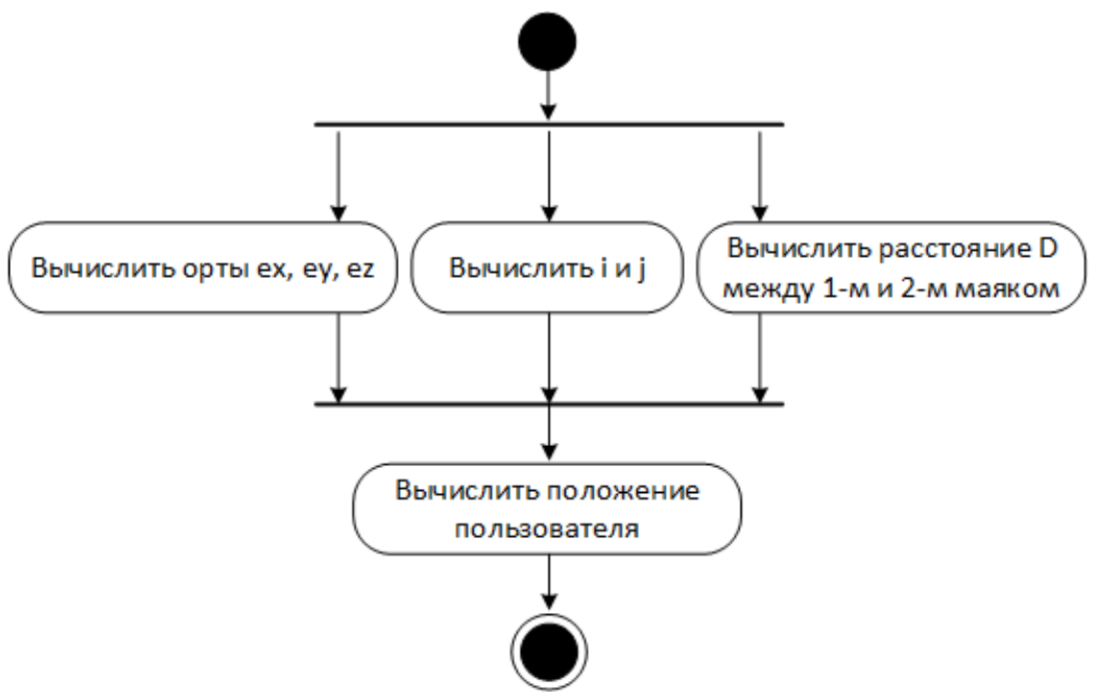
\includegraphics[scale=0.5]{img/sphereIntAct}
    \caption{Activity-диаграмма алгоритма пересечения сфер}
\end{figure}